\lstdefinestyle{yaml}{
     basicstyle=\color{red}\footnotesize,
     rulecolor=\color{black},
     string=[s]{'}{'},
     stringstyle=\color{red},
     comment=[l]{:},
     commentstyle=\color{black},
     morecomment=[l]{-}
 }
 
\chapter{Cloud Computing and Amazon Web Services} \label{ch:CloudComputingAndAmazonWebServices}

As the analysis in previous chapters has shown, the \gls{ac:sdv} is a pivotal advancement in the evolution of the entire automotive industry toward a safer, more efficient, and more sustainable future. Cloud computing is a crucial resource for \gls{ac:sdv} development due to its facilitation of development through its features and benefits. In the following section, cloud computing technologies will be analyzed in detail, focusing on one of the most important providers, \gls{ac:aws}.
\section{Cloud Computing}
The \gls{ac:nist} provides the most comprehensive definition of cloud computing such as: "a model for enabling ubiquitous, convenient, on-demand network access to a shared pool of configurable computing resources (e.g., networks, servers, storage, applications, and services) that can be rapidly provisioned and released with minimal management effort or service provider interaction. This cloud model is composed of five essential characteristics, three service models, and four deployment models" \cite{NISTCloudComputing}. This allows for a thorough analysis of the features of cloud computing in relation to \gls{ac:aws} services, starting with the five essential characteristics.
\begin{itemize}
    \item \textbf{On-demand self-service:} Consumers can access and allocate computing resources autonomously, such as server time and network storage, without direct involvement with service providers. \gls{ac:aws} offers a vast cloud infrastructure with over 200 fully-featured services that consumers can easily access and use from their \gls{ac:aws} account.
    \item \textbf{Broad network access:} Resources can be accessed over the network through standard mechanisms, making them usable across various client platforms. In \gls{ac:aws} services, this is translated as an on-demand delivery of \gls{ac:it} resources over the \textit{Internet} with "pay-as-you-go" pricing. 
    \item \textbf{Resource pooling:} Providers pool computing resources in a multi-tenant model, dynamically assigning them based on consumer demand. As said before \gls{ac:aws} services are allocable e pagabili in base alle necessità del momento. The customer has limited control over the exact resource location but can specify a higher-level abstraction as country, state, or datacenter. In \gls{ac:aws}, clients can select the geographic location of their services through regions. textit{\gls{ac:aws} Regions} provide access to \gls{ac:aws} services that are physically located in a specific geographic area. \gls{ac:aws} provides the option to view the availability of a particular service in a specific region, in addition to selecting different regions \cite{AWSRegions}. Resources include storage, processing, memory, and network bandwidth. It also provides services for the \gls{ac:iot}, machine learning, data lakes, and analytics.
    \item \textbf{Rapid elasticity:} Resources can be easily adjusted to match fluctuations in demand, either automatically or manually. \gls{ac:aws} provides various automated resource allocation systems, including the \gls{ac:aws} \gls{ac:cdk} framework, which will be discussed later. The available capabilities are perceived as virtually limitless, and consumers can acquire them in any quantity at any time, always with a "pay-per-use" system.
    \item \textbf{Measured service:} Cloud systems efficiently manage resources through automated control and optimization, utilizing metering capabilities tailored to specific services such as storage, processing, bandwidth, and user accounts. For instance, \gls{ac:aws} has infrastructure worldwide, allowing for easy deployment of applications in multiple physical locations. The proximity to end-users reduces latency and enhances their experience. This feature allows for clear and objective monitoring, control, and reporting of resource usage by both providers and consumers.
\end{itemize}

The three primary types of cloud computing are \gls{ac:iaas},\gls{ac:paas}, and \gls{ac:saas}. These options provide different levels of control, flexibility, and management, allowing users to configure services to meet their specific requirements.
\begin{itemize}
    \item \textbf{\gls{ac:iaas}:} Consumers are able to utilize and deploy fundamental computing resources, including processing, storage, and networks. However, they only have control over operating systems, storage, and applications, as the cloud infrastructure is managed by the provider. Consumer control over some networking components is limited. \gls{ac:iaas} provides a high level of flexibility and management control over \gls{ac:it} resources. It is similar in practice to existing \gls{ac:it} resources that many \gls{ac:it} departments and developers are already familiar with. 
    \item \textbf{\gls{ac:paas}:} Consumers can deploy their applications on the cloud infrastructure using the programming languages, libraries, services, and tools supported by the provider. The provider manages the underlying cloud infrastructure, including network, servers, operating systems, and storage, while consumers maintain control over their applications and configuration settings. This approach improves efficiency by eliminating the need to manage resource procurement, capacity allocation, software maintenance, patching, or any other tasks involved in running your application. 
    \item \textbf{\gls{ac:saas}:} Consumers can use the provider's applications on the cloud infrastructure, which are accessible from different client devices through interfaces such as web browsers or programs. However, consumers do not have control over the underlying cloud infrastructure, including the network, servers, operating systems, and storage, except for limited user-specific application configuration settings. With a \gls{ac:saas} offering, users do not need to worry about maintaining the service or managing the underlying infrastructure. The focus should be on how to use the software effectively.
\end{itemize}

The analysis thus far has focused on cloud computing, specifically the essential characteristics that a cloud service must possess to be considered a true cloud service, as well as the service models that can be offered. Now, let's analyze in more detail the part related to cloud computing service deployment models and explore which models are most suitable for which workloads using \gls{ac:aws} \cite{AWSPrivatePublicHybrid}. Note that in this case, there are slight differences between the \gls{ac:nist} and \gls{ac:aws} definitions of the various deployment modes.
\begin{itemize}
    \item \textbf{public cloud:} According to \gls{ac:nist}, a public cloud is defined as cloud infrastructure that is publicly accessible and owned, managed, and operated by businesses, academic institutions, government entities, or a combination thereof. In contrast, \gls{ac:aws} defines a public cloud as infrastructure and services that are accessible over the public internet and hosted in a specific \textit{\gls{ac:aws} Region}.
    \item \textbf{private cloud:} Both \gls{ac:nist} and \gls{ac:aws} define private cloud as a cloud infrastructure exclusively provisioned for a single organization, which may own, manage, and operate it independently or in collaboration with a third party. However, there is a difference in the location of the infrastructure. According to \gls{ac:nist}, the infrastructure can be located on or off premises, while in \gls{ac:aws} documentation, the infrastructure is provisioned on premises using a virtualization layer.
    \item \textbf{hybrid cloud:} The hybrid cloud is a combination of two or more separate cloud infrastructures, private or public, connected by technology to facilitate data and application portability. It allows organizations to leverage the cloud for its efficiency and cost savings while also maintaining on-site security, privacy, and control.
\end{itemize}

Exploring the many benefits of cloud computing, the focus now shifts to a comprehensive analysis of the main value patterns of cloud computing, with some charts and graphs to help clarify the outlook.

\begin{table}[h]
    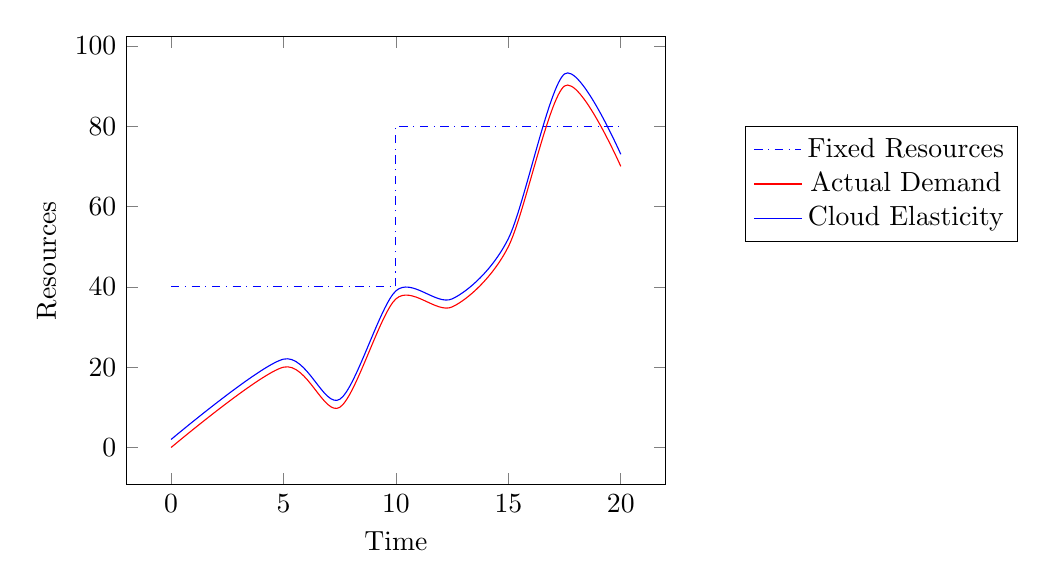
\begin{tikzpicture}
        \begin{axis}[xlabel={Time}, ylabel={Resources}, legend style={at={(1.4,0.8)},anchor=north},]
            % Fixed Resources line
            \addplot[blue,mark=none, dash dot] coordinates {(0,40) (10,40) (10,80) (20,80)};
            \addlegendentry{Fixed Resources}
        
            % Actual Demand line
            \addplot[red,mark=none, smooth] coordinates {(0,0) (5,20) (7.5,10) (10,37) (12.5,35) (15, 50) (17.5, 90) (20, 70)};
            \addlegendentry{Actual Demand}
        
            % Cloud Elasticity line
            \addplot[blue,mark=none, smooth] coordinates {(0,2) (5,22) (7.5,12) (10,39) (12.5,37) (15, 52) (17.5, 93) (20, 73)};
            \addlegendentry{Cloud Elasticity}
        \end{axis}
    \end{tikzpicture}
    \caption{Operating expenditure value model \cite{CloudComputing}}
    \label{tab:OperatingExpenditureValueModel}
\end{table}

Cloud computing reduces costs by aggregating resources needed by different companies in a transparent way to consumers. This means that a company will no longer need to spend excessive amounts of money on building its \gls{ac:it} system to meet overestimated demands or satisfy underestimations of necessary resources as it is shown in \ref{tab:OperatingExpenditureValueModel}.
In addition to shortening the time to market and increasing earnings, cloud computing allows for access to resources anytime and anywhere, optimizing resource management with lower latency and a better experience as it is shown in \ref{tab:LocationFlexibilityValueModel}.

\begin{table}[h]
    \begin{tikzpicture}
        \begin{axis}[xtick={}, xlabel={Location}, ylabel={Availability}, ytick={10,80}, yticklabels={Low, High}, legend style={at={(1.4,0.8)},anchor=north},]
            % Traditional Computing line
            \addplot[blue,mark=none, dash dot] coordinates {(0,10) (5,30) (7.5,35) (10,40) (12.5,35) (15, 50) (17.5, 60) (20, 55)};
            \addlegendentry{Traditional Computing}
        
            % Cloud Computing line
            \addplot[blue,mark=none, smooth,] coordinates {(0,80) (5,80) (10,80) (15, 80) (20, 80)};
            \addlegendentry{Cloud Computing}
        \end{axis}
    \end{tikzpicture}
    \caption{Location flexibility value model \cite{CloudComputing}}
    \label{tab:LocationFlexibilityValueModel}
\end{table}

In conclusion, cloud computing, exemplified by platforms like \gls{ac:aws}, enables organizations to access \gls{ac:it} resources on-demand via the Internet. This is facilitated by pay-as-you-go pricing models, which liberate organizations from the burdens of procuring, owning, and maintaining physical infrastructure. Cloud computing has a wide range of applications across industries, including the automotive sector. One of the main benefits of cloud computing is its dynamic scalability, which improves operational efficiency and reduces costs by utilizing resources more cost-effectively. This is due to the economies of scale inherent in cloud services, resulting in significantly lower variable expenses compared to self-managed infrastructure \cite{AWSWhatIsCloudComputing}. The characteristics of \gls{ac:aws} are analyzed in depth below.

\section{Amazon Web Services}

\gls{ac:aws} is a widely adopted cloud solution with over 200 fully featured services available globally across multiple data centers. It is used by millions of customers, from emerging startups to industry giants and government agencies, as the cloud platform of choice to reduce costs, increase agility, and accelerate innovation \cite{EuAmazonWebServices}.

\gls{ac:aws} stands out by providing a broad set of services, including infrastructure technologies as well as cutting-edge capabilities such as machine learning, artificial intelligence, data lakes, analytics, and the \gls{ac:iot}. This extensive service portfolio facilitates the fast, easy and cost-effective migration of existing applications to the cloud and the creation of diverse digital solutions. \gls{ac:aws} provides purpose-built databases for various application types, allowing users to choose the most suitable tool for optimal cost and performance. The depth of \gls{ac:aws} services is unmatched, providing customers with a comprehensive toolkit for diverse computing needs.

Beyond its vast offerings, \gls{ac:aws} has a large and dynamic global community with millions of active customers and tens of thousands of partners. This inclusive ecosystem spans industries and business sizes, with startups, enterprises, and public sector entities leveraging \gls{ac:aws} for a myriad of use cases. The \gls{ac:apn} solidifies this network with thousands of system integrators and independent software vendors who adapt their technology to work on \gls{ac:aws}.

\gls{ac:aws} demonstrates its commitment to innovation through continuous technological advancements. In 2014, \gls{ac:aws} launched \textit{AWS Lambda}, which pioneered serverless computing. This allows developers to run their code without the need to provision or manage servers. Another example is \textit{Amazon SageMaker}, a fully managed machine learning service that empowers developers to use machine learning without any previous experience.

Rooted in more than 17 years of operational experience, \gls{ac:aws} offers unmatched reliability, security, and performance \cite{WhatIsAWS}. Since its establishment in 2006, \gls{ac:aws} has become a globally trusted platform, revolutionizing \gls{ac:it} infrastructure services by providing a highly reliable, scalable, and cost-effective cloud solution for businesses worldwide in the form of web services with "pay-as-you-go" pricing \cite{AboutAWS}. One of the main advantages of cloud computing is the ability to replace a company's initial capital expenditures required for infrastructure with low costs that vary as needed and can scale with the business. \gls{ac:aws} places great emphasis on the security of its systems and services, which is a fundamental pillar of their platform. In this thesis, we will analyze this feature in more detail.

\subsection{Security}
\gls{ac:aws} is known for its flexible and secure cloud computing environment, designed to meet the strict security requirements of military, global banks, and high-sensitivity organizations. The infrastructure includes over 300 security, compliance, and governance services, supporting 143 security standards and compliance certifications. This architecture ensures scalability, reliability, and rapid deployment of applications and data while adhering to the highest security standards. Strong security at the core of an organization enables digital transformation and innovation. \gls{ac:aws} utilizes redundant controls, continuous testing, and automation to maintain monitoring and protection forever non-stop continuously. Unlike customers' \gls{ac:it} departments, which often operate on limited budgets, \gls{ac:aws} prioritizes security as a core business aspect and allocates significant resources to safeguard the cloud and assist customers in ensuring robust cloud security \cite{AWSCloudComputing}. 

\gls{ac:aws} empowers customers to confidently advance their businesses by providing a secure and innovative cloud infrastructure, a comprehensive suite of security services, and strategic partnerships. The \gls{ac:aws} cloud infrastructure, combined with a comprehensive suite of security services and strategic partnerships, provides a solid foundation for secure innovation. Security is integrated and automated at every level of the organization, ensuring a swift and secure development process while reducing human errors. \gls{ac:aws} offers a wide range of security services and partner solutions to help organizations effectively navigate evolving threats and compliance challenges. These expert-built capabilities equip organizations with the tools they need to stay secure and compliant \cite{AWSSecurity}.

The \gls{ac:aws} global infrastructure follows rigorous security best practices and compliance standards, ensuring that users have access to one of the most secure computing environments in the world. It is designed and managed in alignment with a range of \gls{ac:it} security standards, providing assurance to customers, including those in the life sciences industry, that their web architectures are built on exceptionally secure computing infrastructure. The main security standards obtained from infrastructure will now be explored through \gls{ac:aws} documentation \cite{AWSCertificationsAndAttestations}. 
\begin{itemize}
    \item \textbf{\gls{ac:soc} 1, 2, 3: } \gls{ac:aws} \gls{ac:soc} Reports are third-party examination reports that demonstrate \gls{ac:aws}'s alignment with key compliance controls and objectives. \gls{ac:soc} 1 focuses on controls relevant to a financial audit, covering security organization, access, data handling, change management, and more. \gls{ac:soc} 2 expands to \textit{\gls{ac:aicpa} Trust Services Principles}, evaluating controls related to security, availability, processing integrity, confidentiality, and privacy. The SOC 3 report is a publicly available summary of SOC 2. It includes an external auditor's assessment, \gls{ac:aws} management's assertion, and an overview of \gls{ac:aws} Infrastructure and Services. The report provides transparency and demonstrates \gls{ac:aws}'s commitment to security, compliance, and protection of customer data \cite{AWSSOC3}.
    \begin{figure}[h]  % 'h' significa che la figura viene posizionata qui
        \centering
        
\includegraphics[width=0.4\textwidth]{images/AWSSOC.png}  % Sostituisci 'nome_immagine' con il nome del tuo file immagine e l'estensione
        \caption{\gls{ac:aws} \gls{ac:soc} Logo}
        \label{fig:AWSSOC}
    \end{figure}
    \item \textbf{\gls{ac:fedramp}:} \gls{ac:fedramp} is a United States government program that ensures a standardized approach to security assessment, authorization, and continuous monitoring for cloud products and services. It is aligned with \gls{ac:nist} SP 800 series. The program mandates that cloud service providers undergo an independent security assessment by a \gls{ac:3pao} to verify compliance with the  \gls{ac:fisma} \cite{Fedramp}.
    \item \textbf{\gls{ac:iso} 9001:} "\gls{ac:iso} 9001 is a globally recognized standard for quality management. It helps organizations of all sizes and sectors to improve their performance, meet customer expectations and demonstrate their commitment to quality. Its requirements define how to establish, implement, maintain, and continually improve a \gls{ac:qms}" \cite{ISO9001}. \gls{ac:aws} \gls{ac:iso} 9001:2015 certification directly supports customers developing, migrating, and operating their quality-controlled \gls{ac:it} systems in the \gls{ac:aws} cloud. They can use \gls{ac:aws} compliance reports as evidence for their own \gls{ac:iso} 9001:2015 programs and industry-specific quality programs \cite{AWSISO9001}.
    \item \textbf{\gls{ac:iso}/\gls{ac:iec} 27001:} \gls{ac:iso}/\gls{ac:iec} 27001 is a global security standard that outlines requirements for the systematic management of corporate and customer information. \gls{ac:aws} has achieved \gls{ac:iso} 27001 certification, demonstrating a comprehensive approach to assessing, managing, and mitigating information security risks. The certification covers \gls{ac:aws} infrastructure, data centers, and services, ensuring ongoing compliance with international security standards \cite{ISOIEC27001}.
    \item \textbf{\gls{ac:iso}/\gls{ac:iec} 27017:} "\gls{ac:iso}/\gls{ac:iec} 27017:2015 gives guidelines for information security controls applicable to the provision and use of cloud services by providing: additional implementation guidance for relevant controls specified in ISO/IEC 27002; additional controls with implementation guidance that specifically relate to cloud services. This Recommendation | International Standard provides controls and implementation guidance for both cloud service providers and cloud service customers" \cite{ISOIEC27017}. This certification ensures the implementation of precise, cloud-specific controls and validates \gls{ac:aws} commitment to robust security measures in cloud services \cite{AWSISOIEC27017}.
    \item \textbf{\gls{ac:iso}/\gls{ac:iec} 27018:} \gls{ac:iso} 27018 is a global code of practice for safeguarding personal data in the cloud. It builds upon \gls{ac:iso} 27002 and offers guidance on implementing controls for \gls{ac:pii} in public clouds. \gls{ac:aws}'s \gls{ac:iso} 27018 certification affirms its dedication to internationally recognized standards, emphasizing privacy and content protection through the use of this certification\cite{AWSISOIEC27018}.
    \item \textbf{\gls{ac:hitrust}:} The \gls{ac:hitrust} integrates global standards such as \gls{ac:gdpr}, \gls{ac:iso}, \gls{ac:nist}, \gls{ac:pci}, and \gls{ac:hipaa} to establish a comprehensive framework for security and privacy controls. Some \gls{ac:aws} services have been assessed under the \gls{ac:hitrust} CSF Assurance Program by an approved \textit{\gls{ac:hitrust} Assessor} and have been found to meet the \textit{\gls{ac:hitrust} Certification Criteria}. Customers can inherit \gls{ac:aws} certification for controls relevant to their cloud architectures established under the \textit{\gls{ac:hitrust} \gls{ac:srm}}. The certification is valid for two years, describes the \gls{ac:aws} services that have been validated, and can be publicly accessed \cite{AWSHITRUSTCSF}.
    \item \textbf{\gls{ac:star}:} The \gls{ac:csa} introduced the \gls{ac:star} to promote transparency in cloud provider security practices. \gls{ac:star} is a publicly accessible registry that documents the security controls of cloud computing offerings. \gls{ac:aws} has joined the \textit{\gls{ac:csa} \gls{ac:star} Self-Assessment}, aligning with \gls{ac:csa} best practices. The completed \textit{\gls{ac:csa} \gls{ac:caiq}} reports for \gls{ac:aws} are publicly available \cite{AWSCSA}.
\end{itemize}

